\documentclass[aspectratio=169, 10pt]{beamer}

% ---------- Tema y colores ----------
\usetheme{default}
\usecolortheme{default}
\setbeamertemplate{navigation symbols}{}
\setbeamertemplate{footline}[frame number]
\setbeamertemplate{frametitle continuation}{}

\definecolor{StanfordRed}{RGB}{140,21,21}
\definecolor{LightGray}{RGB}{240,240,240}
\definecolor{AccentGreen}{RGB}{0,130,100}
\definecolor{UCMBlue}{RGB}{4, 171, 226}
\definecolor{UCMNavy}{RGB}{20, 65, 134}

\definecolor{mitblue}{RGB}{20, 65, 134}
\definecolor{mitgray}{RGB}{169, 169, 169}

\setbeamercolor{frametitle}{fg=white, bg=UCMBlue}
\setbeamercolor{title}{fg=white}
\setbeamercolor{author}{fg=white}
\setbeamercolor{institute}{fg=white!80}
\setbeamercolor{structure}{fg=UCMBlue}
\setbeamercolor{block title}{bg=UCMBlue!15!white, fg=UCMBlue}
\setbeamercolor{block body}{bg=LightGray}
\setbeamercolor{block title alerted}{bg=StanfordRed!15!white, fg=StanfordRed}
\setbeamercolor{block body alerted}{bg=LightGray}
\setbeamercolor{alerted text}{fg=UCMBlue}

\setbeamerfont{frametitle}{series=\bfseries, size=\large}
\setbeamerfont{title}{series=\bfseries, size=\LARGE}
\setbeamerfont{block title}{series=\bfseries}

% ---------- Paquetes ----------
\usepackage[utf8]{inputenc}
\usepackage[T1]{fontenc}
\usepackage[provide=*,spanish]{babel}
\usepackage{amsmath, amssymb}
\usepackage{graphicx}
\usepackage{tikz}
\usepackage{pgfplots}
\pgfplotsset{compat=1.18}
\usetikzlibrary{arrows, arrows.meta, shapes, shapes.geometric, positioning,
	fit, calc, matrix, chains, decorations.pathreplacing,
	backgrounds, shadows}
\usepackage{booktabs}
\usepackage{array}
\usepackage{xcolor}
\usepackage{multicol}
\usepackage{tcolorbox}
\tcbuselibrary{skins, breakable}
\usepackage{fontawesome5}

% ---------- Comandos útiles ----------
\providecommand{\R}{\mathbb{R}}
\newcommand{\Q}{\mathbf{Q}}
\newcommand{\K}{\mathbf{K}}
\newcommand{\Vm}{\mathbf{V}}
\newcommand{\qv}{\mathbf{q}}
\newcommand{\kv}{\mathbf{k}}
\newcommand{\vv}{\mathbf{v}}
\newcommand{\softmax}{\mathrm{softmax}}
\newcommand{\good}{{\color{AccentGreen}\faCheck}}
\newcommand{\bad}{{\color{StanfordRed}\faTimes}}

\newcommand{\formula}[1]{%
	\begin{tcolorbox}[colback=UCMBlue!8, colframe=UCMBlue, arc=4pt,
		boxsep=2pt, left=6pt, right=6pt, top=3pt, bottom=3pt]
		#1
	\end{tcolorbox}
}

% bloque genérico para diagramas
\tikzset{
	box/.style={draw=UCMNavy, fill=mitblue!15, rounded corners=2pt, minimum height=0.6cm,
		minimum width=2.6cm, font=\scriptsize, align=center},
	smallbox/.style={draw=UCMNavy, fill=white, rounded corners=2pt, minimum height=0.5cm,
		font=\scriptsize, align=center},
	arr/.style={-{Stealth[length=2mm]}, thick, UCMNavy},
}

% ---------- Portada ----------
\title{\textbf{Atenci\'on y la Arquitectura Transformer}}
\subtitle{De la atenci\'on de Bahdanau a los modelos de lenguaje masivos}
\author{Sergio Hern\'andez, PhD\\ shernandez@ucm.cl}
\institute{
	\begin{tikzpicture}[scale=0.42, every node/.style={transform shape}]
		\foreach \i/\y in {1/0,2/1,3/2}{\node[circle,draw=white,fill=white!20,minimum size=4mm] (i\i) at (0,\y){};}
		\foreach \i/\y in {1/-0.5,2/0.5,3/1.5,4/2.5}{\node[circle,draw=white,fill=white!35,minimum size=4mm] (h\i) at (2,\y){};}
		\foreach \i/\y in {1/0.5,2/1.5}{\node[circle,draw=white,fill=white!50,minimum size=4mm] (o\i) at (4,\y){};}
		\foreach \a in {1,2,3}\foreach \b in {1,2,3,4}{\draw[white,opacity=0.5] (i\a)--(h\b);}
		\foreach \a in {1,2,3,4}\foreach \b in {1,2}{\draw[white,opacity=0.5] (h\a)--(o\b);}
	\end{tikzpicture}
	\\ \textbf{Mag\'ister en Data Science --- Universidad Cat\'olica del Maule}}
\date{}

\begin{document}
% --- Título ---
{
	\setbeamertemplate{background}{
		\begin{tikzpicture}[remember picture, overlay]
			\fill[UCMBlue] (current page.south west) rectangle (current page.north east);
			\fill[UCMBlue!70!black, opacity=0.5]
			(current page.south west) -- ++(0,3) -- ++(18,0) -- cycle;
			\foreach \i in {1,...,40}{
				\fill[white, opacity=0.04]
				({random()*17}, {random()*10}) circle ({random()*0.3});
			}
		\end{tikzpicture}
	}
	\begin{frame}[plain]
		\vspace{1.2cm}
		\titlepage
		\begin{tikzpicture}[remember picture, overlay]
			\node[white, opacity=0.18, font=\fontsize{28}{28}\selectfont, anchor=south east]
			at (current page.south east) [xshift=-0.6cm, yshift=0.5cm] {$\softmax\!\left(\frac{\mathbf{Q}\mathbf{K}^{\top}}{\sqrt d}\right)\!\mathbf{V}$};
		\end{tikzpicture}
	\end{frame}
}

% =================================================================
\section{Introducci\'on}

\begin{frame}{¿D\'onde Estamos?}
	\begin{columns}[T]
		\begin{column}{0.5\textwidth}
			\begin{block}{Clase 3.2}
				\small
				\begin{itemize}
					\item Embeddings vectoriales.
					\item RNN, LSTM y GRU: procesan la secuencia \textbf{paso a paso}.
					\item Arquitectura codificador--decodificador (seq2seq).
				\end{itemize}
			\end{block}
			\begin{alertblock}{Dos problemas de las RNN}
				\small
				\begin{enumerate}
					\item \textbf{Cuello de botella}: toda la fuente se comprime en un \'unico estado de tama\~no fijo.
					\item \textbf{Secuencialidad}: el paso $t$ espera al paso $t-1$; no se paraleliza en GPU.
				\end{enumerate}
			\end{alertblock}
		\end{column}
		\begin{column}{0.47\textwidth}
			\begin{block}{Esta clase}
				\small
				\begin{enumerate}
					\item Consultas, claves y valores.
					\item Atenci\'on por similitud (Nadaraya--Watson).
					\item Funciones de puntaje y \emph{masked softmax}.
					\item Atenci\'on de Bahdanau.
					\item Auto-atenci\'on: simple, con pesos entrenables y causal.
					\item Atenci\'on multi-cabeza.
					\item Codificaci\'on posicional.
					\item El Transformer.
					\item Vision Transformer.
					\item Preentrenamiento: BERT, T5, GPT.
					\item Laboratorio 3.3.
				\end{enumerate}
			\end{block}
		\end{column}
	\end{columns}
	\vfill
	{\scriptsize Contenido basado en \emph{Dive into Deep Learning}, cap.\ 11 (d2l.ai).}
\end{frame}

\begin{frame}{El Cuello de Botella del Modelo Seq2Seq}
	\begin{center}
		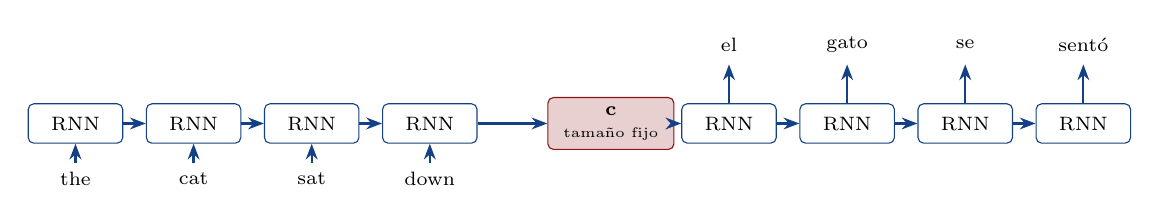
\begin{tikzpicture}[x=1cm,y=1cm]
			% encoder
			\foreach \i/\w in {1/{the},2/{cat},3/{sat},4/{down}}{
				\node[smallbox, minimum width=1.2cm] (e\i) at (\i*1.5,0) {RNN};
				\node[font=\scriptsize] at (\i*1.5,-0.7) {\w};
				\draw[arr] (\i*1.5,-0.5)--(e\i.south);
			}
			\foreach \i/\j in {1/2,2/3,3/4}{\draw[arr] (e\i)--(e\j);}
			% context
			\node[box, fill=StanfordRed!20, draw=StanfordRed, minimum width=1.6cm] (c) at (8.3,0) {$\mathbf{c}$\\ \tiny tama\~no fijo};
			\draw[arr] (e4)--(c);
			% decoder
			\foreach \i/\w in {1/{el},2/{gato},3/{se},4/{sent\'o}}{
				\node[smallbox, minimum width=1.2cm] (d\i) at (8.3+\i*1.5,0) {RNN};
				\node[font=\scriptsize] at (8.3+\i*1.5,1.0) {\w};
				\draw[arr] (d\i.north)--(8.3+\i*1.5,0.75);
			}
			\draw[arr] (c)--(d1);
			\foreach \i/\j in {1/2,2/3,3/4}{\draw[arr] (d\i)--(d\j);}
		\end{tikzpicture}
	\end{center}
	\begin{itemize}
		\item Toda la oraci\'on fuente debe caber en $\mathbf{c}\in\R^h$, sin importar su largo.
		\item El rendimiento cae al aumentar la longitud de la entrada.
		\item \textbf{Idea} (Bahdanau, Cho y Bengio, 2014): en cada paso del decodificador, \emph{mirar} los estados del codificador que sean relevantes en lugar de depender de un \'unico vector.
	\end{itemize}
\end{frame}

% =================================================================
\section{Atenci\'on: Consultas, Claves y Valores}

\begin{frame}{Consultas, Claves y Valores}
	\begin{columns}[T]
		\begin{column}{0.52\textwidth}
			Una \textbf{base de datos} de $m$ pares clave--valor:
			\[
			\mathcal{D}=\{(\kv_1,\vv_1),\dots,(\kv_m,\vv_m)\}
			\]
			y una \textbf{consulta} $\qv$.

			\medskip
			\formula{
				\[
				\mathrm{Attention}(\qv,\mathcal{D})=\sum_{i=1}^{m}\alpha(\qv,\kv_i)\,\vv_i
				\]
			}
			\begin{itemize}
				\item $\alpha(\qv,\kv_i)\in\R$: \textbf{pesos de atenci\'on}.
				\item La operaci\'on se llama \emph{attention pooling}.
				\item Es una selecci\'on \textbf{diferenciable} sobre un conjunto de tama\~no variable.
			\end{itemize}
		\end{column}
		\begin{column}{0.45\textwidth}
			\begin{center}
				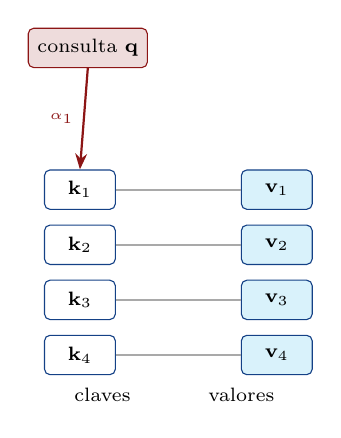
\begin{tikzpicture}[x=1cm,y=1cm]
					\node[smallbox, fill=StanfordRed!15, draw=StanfordRed] (q) at (0,2) {consulta $\qv$};
					\foreach \i/\y in {1/0.9,2/0.2,3/-0.5,4/-1.2}{
						\node[smallbox, minimum width=0.9cm] (k\i) at (-0.1,\y-0.7) {$\kv_\i$};
						\node[smallbox, fill=UCMBlue!15, minimum width=0.9cm] (v\i) at (2.4,\y-0.7) {$\vv_\i$};
						\draw[thick, mitgray] (k\i)--(v\i);
					}
					\draw[arr, StanfordRed] (q.south)--(k1.north) node[midway,left,font=\tiny]{$\alpha_1$};
					\node[font=\scriptsize] at (1.1,-2.4) {claves \hspace{0.8cm} valores};
				\end{tikzpicture}
			\end{center}
		\end{column}
	\end{columns}
\end{frame}

\begin{frame}{Normalizaci\'on y Casos Especiales}
	Para que los pesos formen una combinaci\'on convexa se aplica \textbf{softmax} a una funci\'on de puntaje $a(\qv,\kv)$:
	\formula{
		\[
		\alpha(\qv,\kv_i)=\frac{\exp\big(a(\qv,\kv_i)\big)}{\sum_{j=1}^{m}\exp\big(a(\qv,\kv_j)\big)}
		\qquad \alpha_i\ge 0,\ \ \sum_i\alpha_i=1
		\]
	}
	\begin{columns}[T]
		\begin{column}{0.48\textwidth}
			\begin{block}{Casos especiales}
				\small
				\begin{itemize}
					\item Un peso $=1$ y el resto $0$: consulta cl\'asica a una base de datos.
					\item Todos los pesos $=1/m$: \emph{average pooling}.
					\item Pesos no negativos: la salida est\'a en el cono convexo de los valores.
				\end{itemize}
			\end{block}
		\end{column}
		\begin{column}{0.48\textwidth}
			\begin{block}{¿Por qu\'e softmax?}
				\small
				\begin{itemize}
					\item Es diferenciable y sus gradientes no se anulan.
					\item La atenci\'on no diferenciable (selecci\'on dura) requiere aprendizaje por refuerzo.
					\item Todos los mecanismos de atenci\'on populares usan softmax.
				\end{itemize}
			\end{block}
		\end{column}
	\end{columns}
\end{frame}

\begin{frame}{Atenci\'on por Similitud: Regresi\'on de Nadaraya--Watson}
	Precursor de la atenci\'on (1964): un promedio de las salidas observadas, ponderado por un \textbf{n\'ucleo} (kernel).
	\formula{
		\[
		f(x)=\sum_{i=1}^{n}\frac{K(x-x_i)}{\sum_{j}K(x-x_j)}\,y_i
		\]
	}
	\vspace{-0.3cm}
	\begin{columns}[T]
		\begin{column}{0.5\textwidth}
			\begin{block}{En lenguaje de atenci\'on}
				\small
				\begin{itemize}
					\item \textbf{consulta} = punto donde se predice
					\item \textbf{claves} = entradas observadas $x_i$
					\item \textbf{valores} = salidas observadas $y_i$
				\end{itemize}
			\end{block}
			\small
			No requiere entrenamiento. Para clasificaci\'on, $\vv_i$ es el one-hot de $y_i$.
		\end{column}
		\begin{column}{0.48\textwidth}
			\begin{center}
				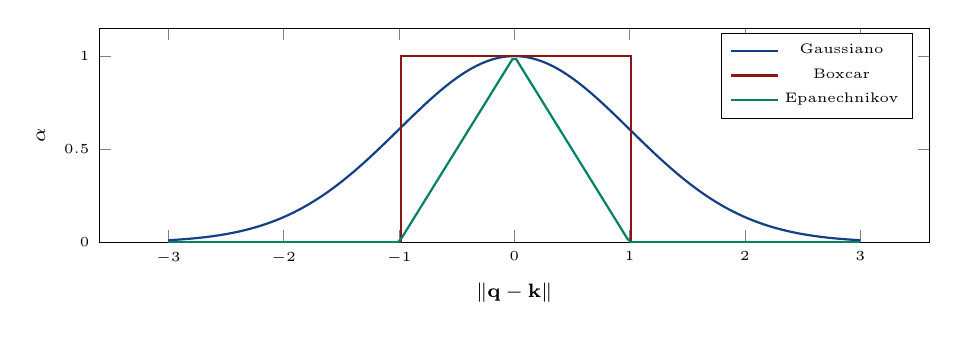
\begin{tikzpicture}
					\begin{axis}[width=\textwidth, height=4.3cm, xlabel={$\|\qv-\kv\|$}, ylabel={$\alpha$},
						legend style={font=\tiny, at={(0.98,0.98)}, anchor=north east},
						domain=-3:3, samples=200, ymin=0, ymax=1.15, tick label style={font=\tiny},
						label style={font=\scriptsize}]
						\addplot[thick, UCMNavy] {exp(-x^2/2)};
						\addplot[thick, StanfordRed, const plot, samples=400] {abs(x)<=1 ? 1 : 0};
						\addplot[thick, AccentGreen] {max(0, 1-abs(x))};
						\legend{Gaussiano, Boxcar, Epanechnikov}
					\end{axis}
				\end{tikzpicture}
			\end{center}
		\end{column}
	\end{columns}
\end{frame}

\begin{frame}{Nadaraya--Watson: Qu\'e Observar}
	Experimento de d2l: $y_i=2\sin(x_i)+x_i+\epsilon$, $\epsilon\sim\mathcal{N}(0,1)$, 40 puntos en $[0,5]$.
	\begin{columns}[T]
		\begin{column}{0.5\textwidth}
			\begin{itemize}
				\item Gaussiano, boxcar y Epanechnikov dan ajustes similares.
				\item N\'ucleo \textbf{constante}: se reduce a la media global de $y$.
				\item Ancho menor: curva menos suave, sigue mejor la variaci\'on local.
				\item Un ancho fijo no es \'optimo en todas partes (heur\'istica de Silverman para anchos adaptativos).
			\end{itemize}
		\end{column}
		\begin{column}{0.47\textwidth}
			\begin{alertblock}{Limitaci\'on}
				La similitud est\'a \textbf{fijada a mano}. En deep learning queremos \emph{aprender} las representaciones de consultas y claves para que la similitud sea \'util para la tarea.
			\end{alertblock}
			\begin{block}{Siguiente paso}
				Reemplazar $\|\qv-\kv\|$ por una funci\'on de puntaje parametrizada.
			\end{block}
		\end{column}
	\end{columns}
\end{frame}

% =================================================================
\section{Funciones de Puntaje}

\begin{frame}{De Distancia Gaussiana a Producto Punto}
	Puntaje gaussiano, expandido:
	\formula{
		\[
		a(\qv,\kv_i)=-\tfrac12\|\qv-\kv_i\|^2
		=\qv^\top\kv_i-\tfrac12\|\kv_i\|^2-\tfrac12\|\qv\|^2
		\]
	}
	\begin{itemize}
		\item $\tfrac12\|\qv\|^2$ es igual para todas las claves: se cancela en el softmax.
		\item $\tfrac12\|\kv_i\|^2$ suele ser casi constante (p.\,ej.\ tras normalizaci\'on en capas anteriores) y se descarta.
		\item Queda el \textbf{producto punto} $\qv^\top\kv_i$: la similitud mide alineamiento.
	\end{itemize}
	\begin{block}{Dos opciones populares}
		\small
		\begin{enumerate}
			\item \textbf{Producto punto escalado}: eficiente (una multiplicaci\'on de matrices); exige dimensiones iguales de $\qv$ y $\kv$.
			\item \textbf{Atenci\'on aditiva}: permite consultas y claves de dimensiones distintas.
		\end{enumerate}
	\end{block}
\end{frame}

\begin{frame}{Producto Punto Escalado}
	\formula{
		\[
		a(\qv,\kv_i)=\frac{\qv^\top\kv_i}{\sqrt d}
		\qquad\Longrightarrow\qquad
		\boxed{\ \mathrm{Attention}(\Q,\K,\Vm)=\softmax\!\left(\frac{\Q\K^\top}{\sqrt d}\right)\Vm\ }
		\]
	}
	con $\Q\in\R^{n\times d}$, $\K\in\R^{m\times d}$, $\Vm\in\R^{m\times v}$ y salida en $\R^{n\times v}$.
	\begin{columns}[T]
		\begin{column}{0.5\textwidth}
			\begin{block}{¿Por qu\'e dividir por $\sqrt d$?}
				\small
				Si las componentes de $\qv$ y $\kv$ son independientes con media 0 y varianza 1, entonces $\qv^\top\kv$ tiene varianza $d$. Dividir por $\sqrt d$ la devuelve a 1.
				Sin esto, para $d$ grande el softmax se satura (un peso $\approx1$) y los gradientes casi se anulan.
			\end{block}
		\end{column}
		\begin{column}{0.47\textwidth}
			\begin{center}
				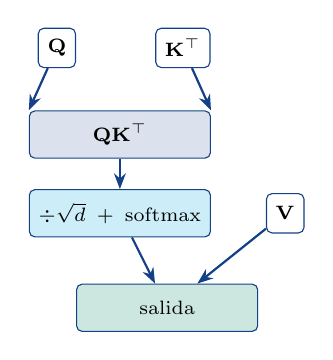
\begin{tikzpicture}[x=1cm,y=1cm]
					\node[smallbox] (Q) at (0,1.6) {$\Q$};
					\node[smallbox] (K) at (1.6,1.6) {$\K^\top$};
					\node[box, minimum width=2.3cm] (M) at (0.8,0.5) {$\Q\K^\top$};
					\node[box, minimum width=2.3cm, fill=UCMBlue!20] (S) at (0.8,-0.5) {$\div\sqrt d$ \,+\, softmax};
					\node[smallbox] (V) at (2.9,-0.5) {$\Vm$};
					\node[box, minimum width=2.3cm, fill=AccentGreen!20] (O) at (1.4,-1.7) {salida};
					\draw[arr] (Q)--(M.north west); \draw[arr] (K)--(M.north east);
					\draw[arr] (M)--(S); \draw[arr] (S)--(O); \draw[arr] (V)--(O);
				\end{tikzpicture}
			\end{center}
		\end{column}
	\end{columns}
\end{frame}

\begin{frame}{Atenci\'on Aditiva}
	Cuando $\qv\in\R^{q}$ y $\kv\in\R^{k}$ tienen dimensiones distintas:
	\formula{
		\[
		a(\qv,\kv)=\mathbf{w}_v^\top\tanh\!\big(\mathbf{W}_q\qv+\mathbf{W}_k\kv\big)\in\R
		\]
	}
	\begin{columns}[T]
		\begin{column}{0.5\textwidth}
			\begin{itemize}
				\item $\mathbf{W}_q\in\R^{h\times q}$, $\mathbf{W}_k\in\R^{h\times k}$, $\mathbf{w}_v\in\R^{h}$: par\'ametros aprendibles.
				\item Equivale a un MLP de una capa oculta (tanh) sobre la concatenaci\'on de $\qv$ y $\kv$.
				\item Es el puntaje usado originalmente por Bahdanau.
			\end{itemize}
		\end{column}
		\begin{column}{0.47\textwidth}
			\begin{center}
				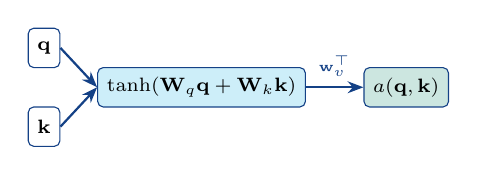
\begin{tikzpicture}[x=1cm,y=1cm]
					\node[smallbox] (q) at (0,0) {$\qv$};
					\node[smallbox] (k) at (0,-1) {$\kv$};
					\node[smallbox, fill=UCMBlue!20] (h) at (2,-0.5) {$\tanh(\mathbf{W}_q\qv+\mathbf{W}_k\kv)$};
					\node[smallbox, fill=AccentGreen!20] (a) at (4.6,-0.5) {$a(\qv,\kv)$};
					\draw[arr] (q.east)--(h.west); \draw[arr] (k.east)--(h.west);
					\draw[arr] (h)--(a) node[midway,above,font=\tiny]{$\mathbf{w}_v^\top$};
				\end{tikzpicture}
			\end{center}
		\end{column}
	\end{columns}
\end{frame}

\begin{frame}{Masked Softmax: Secuencias de Largo Variable}
	En un minibatch las secuencias se rellenan (\emph{padding}); esas posiciones no deben recibir atenci\'on.
	\begin{columns}[T]
		\begin{column}{0.5\textwidth}
			\begin{itemize}
				\item Se reciben las longitudes v\'alidas por ejemplo (1-D) o por consulta (2-D).
				\item Las posiciones inv\'alidas reciben un puntaje muy negativo ($\approx-10^{6}$) antes del softmax $\Rightarrow$ peso $=0$.
				\item Despu\'es del softmax se aplica \emph{dropout} y luego se multiplica por $\Vm$.
			\end{itemize}
		\end{column}
		\begin{column}{0.47\textwidth}
			\begin{center}
				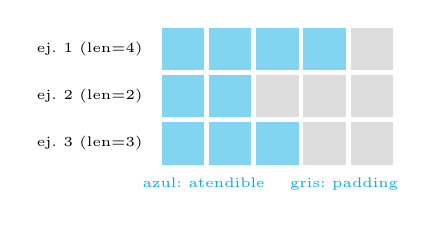
\begin{tikzpicture}[x=0.6cm,y=0.6cm]
					\foreach \r/\n in {0/4,1/2,2/3}{
						\foreach \c in {0,...,4}{
							\ifnum\c<\n
								\fill[UCMBlue!50] (\c,-\r) rectangle ++(0.9,-0.9);
							\else
								\fill[mitgray!40] (\c,-\r) rectangle ++(0.9,-0.9);
							\fi
						}
						\node[font=\tiny, anchor=east] at (-0.2,-\r-0.45) {ej.~\the\numexpr\r+1\relax\ (len=\n)};
					}
					\node[font=\tiny, UCMBlue] at (2.3,-3.3) {azul: atendible \quad gris: padding};
				\end{tikzpicture}
			\end{center}
		\end{column}
	\end{columns}
\end{frame}

\begin{frame}[fragile]{Atenci\'on de Producto Punto en PyTorch}
	\small
	\begin{tcolorbox}[colback=LightGray, colframe=UCMNavy, arc=3pt, boxsep=1pt]
\begin{verbatim}
def masked_softmax(scores, valid_lens):          # scores: (B, Q, K)
    mask = torch.arange(scores.shape[-1])[None, None, :] \
           < valid_lens[:, None, None]
    return torch.softmax(scores.masked_fill(~mask, -1e6), dim=-1)

def attention(Q, K, V, valid_lens=None):
    d = Q.shape[-1]
    scores = Q @ K.transpose(1, 2) / math.sqrt(d)  # (B, n, m)
    weights = masked_softmax(scores, valid_lens)
    return weights @ V, weights                    # (B, n, v)
\end{verbatim}
	\end{tcolorbox}
	\begin{itemize}
		\item \texttt{@} sobre tensores 3-D es una multiplicaci\'on de matrices por lote (\emph{bmm}).
		\item Todo es diferenciable: se entrena con retropropagaci\'on.
	\end{itemize}
\end{frame}

% =================================================================
\section{Atenci\'on de Bahdanau}

\begin{frame}{Atenci\'on de Bahdanau: Contexto Din\'amico}
	El contexto $\mathbf{c}_{t'}$ se recalcula en \textbf{cada} paso $t'$ del decodificador.
	\formula{
		\[
		\mathbf{c}_{t'}=\sum_{t=1}^{T}\alpha(\mathbf{s}_{t'-1},\mathbf{h}_t)\,\mathbf{h}_t,
		\qquad
		\alpha(\mathbf{s},\mathbf{h}_t)=\softmax_t\Big(\mathbf{w}_v^\top\tanh(\mathbf{W}_q\mathbf{s}+\mathbf{W}_k\mathbf{h}_t)\Big)
		\]
	}
	\begin{columns}[T]
		\begin{column}{0.4\textwidth}
			\begin{block}{Roles}
				\small
				\begin{itemize}
					\item \textbf{consulta}: estado previo del decodificador $\mathbf{s}_{t'-1}$
					\item \textbf{claves y valores}: estados del codificador $\mathbf{h}_1,\dots,\mathbf{h}_T$
				\end{itemize}
			\end{block}
			\small
			Entrada del decodificador: $[\mathrm{Embed}(y_{t'-1});\,\mathbf{c}_{t'}]\to$ GRU $\to$ capa densa $\to$ logits del vocabulario.
		\end{column}
		\begin{column}{0.58\textwidth}
			\begin{center}
				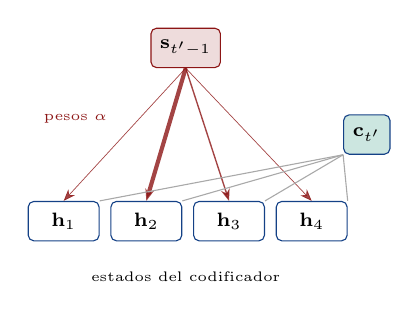
\begin{tikzpicture}[x=1cm,y=1cm]
					\foreach \i in {1,2,3,4}{
						\node[smallbox, minimum width=0.9cm] (h\i) at (\i*1.05,0) {$\mathbf{h}_\i$};
					}
					\node[smallbox, fill=StanfordRed!15, draw=StanfordRed] (s) at (2.6,2.2) {$\mathbf{s}_{t'-1}$};
					\node[smallbox, fill=AccentGreen!20] (c) at (4.9,1.1) {$\mathbf{c}_{t'}$};
					\foreach \i/\w in {1/0.1,2/0.6,3/0.2,4/0.1}{
						\draw[-{Stealth[length=1.5mm]}, StanfordRed, line width={\w*2.5pt}, opacity=0.8] (s.south)--(h\i.north);
					}
					\foreach \i in {1,2,3,4}{\draw[mitgray] (h\i.north east) -- (c.south west);}
					\node[font=\tiny, StanfordRed] at (1.2,1.3) {pesos $\alpha$};
					\node[font=\tiny] at (2.6,-0.7) {estados del codificador};
				\end{tikzpicture}
			\end{center}
		\end{column}
	\end{columns}
\end{frame}

\begin{frame}{Bahdanau: Arquitectura y Entrenamiento}
	\begin{columns}[T]
		\begin{column}{0.5\textwidth}
			\begin{block}{Componentes}
				\small
				\begin{itemize}
					\item \textbf{Codificador}: RNN que entrega los estados de todos los pasos.
					\item \textbf{Atenci\'on}: aditiva, con el estado previo del decodificador como consulta.
					\item \textbf{Decodificador}: embedding $\to$ atenci\'on $\to$ concatenar $\to$ GRU $\to$ densa.
					\item Las \emph{longitudes v\'alidas} de la fuente enmascaran el padding.
				\end{itemize}
			\end{block}
		\end{column}
		\begin{column}{0.47\textwidth}
			\begin{block}{Configuraci\'on en d2l (EN$\to$FR)}
				\small
				\begin{itemize}
					\item Batch 128, embedding y oculta 256, 2 capas, dropout 0.2.
					\item lr $=0.005$, 30 \'epocas, recorte de gradiente 1.
					\item Evaluaci\'on: BLEU.
				\end{itemize}
			\end{block}
			\begin{alertblock}{Lectura de los pesos}
				\small
				Los mapas de calor muestran qu\'e palabras fuente se miran al generar cada palabra objetivo: \textbf{alineamiento} aprendido sin supervisi\'on.
			\end{alertblock}
		\end{column}
	\end{columns}
\end{frame}

% =================================================================
\section{Auto-Atenci\'on}

\begin{frame}{Auto-Atenci\'on Simple (sin Pesos Entrenables)}
	Cada token $\mathbf{x}_i$ se reemplaza por un \textbf{vector de contexto} $\mathbf{z}_i$: una mezcla de \emph{todos} los tokens de la misma secuencia.
	\formula{
		\small
		\[
		\omega_{ij}=\mathbf{x}_i^\top\mathbf{x}_j
		\ \Rightarrow\
		\alpha_{ij}=\frac{e^{\omega_{ij}}}{\sum_{l}e^{\omega_{il}}}
		\ \Rightarrow\
		\mathbf{z}_i=\sum_{j=1}^{n}\alpha_{ij}\mathbf{x}_j
		\qquad\Longleftrightarrow\qquad
		\mathbf{Z}=\softmax(\mathbf{X}\mathbf{X}^\top)\,\mathbf{X}
		\]
	}
	\vspace{-0.2cm}
	\begin{columns}[T]
		\begin{column}{0.5\textwidth}
			\small
			Ejemplo del laboratorio: \emph{Your journey starts with one step}, con embeddings de 3 dimensiones. Consulta: \texttt{journey}.
			\begin{center}
				\scriptsize
				\begin{tabular}{lcccccc}
					\toprule
					& Your & journey & starts & with & one & step\\
					\midrule
					$\omega_{2j}$ & 0.954 & 1.495 & 1.475 & 0.843 & 0.707 & 1.087\\
					$\alpha_{2j}$ & 0.139 & 0.238 & 0.233 & 0.124 & 0.108 & 0.158\\
					\bottomrule
				\end{tabular}
			\end{center}
			$\mathbf{z}_2=(0.442,\ 0.652,\ 0.568)$
		\end{column}
		\begin{column}{0.47\textwidth}
			\begin{alertblock}{Limitaciones}
				\small
				\begin{itemize}
					\item No hay nada que aprender: la similitud depende solo de los embeddings de entrada.
					\item Cada token se atiende mucho a s\'i mismo ($\mathbf{x}\cdot\mathbf{x}$ suele ser el mayor producto punto).
				\end{itemize}
			\end{alertblock}
			\small
			\textbf{Siguiente paso:} proyecciones aprendibles.
		\end{column}
	\end{columns}
\end{frame}

\begin{frame}[fragile]{Auto-Atenci\'on con Pesos Entrenables}
	Tres proyecciones aprendibles dan los roles de \textbf{consulta}, \textbf{clave} y \textbf{valor} (la formulaci\'on QKV de esta clase):
	\formula{
		\small
		\[
		\mathbf{Q}=\mathbf{X}\mathbf{W}_q,\quad \mathbf{K}=\mathbf{X}\mathbf{W}_k,\quad \mathbf{V}=\mathbf{X}\mathbf{W}_v,
		\qquad
		\mathbf{Z}=\softmax\!\left(\frac{\mathbf{Q}\mathbf{K}^\top}{\sqrt{d_k}}\right)\mathbf{V}
		\]
	}
	\vspace{-0.1cm}
	\begin{columns}[T]
		\begin{column}{0.46\textwidth}
			\small
			\begin{itemize}
				\item $\mathbf{X}\in\R^{n\times d_\text{in}}$, $\ \mathbf{W}_{q,k,v}\in\R^{d_\text{in}\times d_\text{out}}$.
				\item \texttt{SelfAttention\_v1}: \texttt{nn.Parameter(torch.rand(...))}.
				\item \texttt{SelfAttention\_v2}: \texttt{nn.Linear}, con sesgo opcional y \textbf{mejor inicializaci\'on}; es la forma est\'andar.
				\item El factor $1/\sqrt{d_k}$ evita que el softmax se sature.
			\end{itemize}
		\end{column}
		\begin{column}{0.53\textwidth}
			\scriptsize
			\begin{tcolorbox}[colback=LightGray, colframe=UCMNavy, arc=3pt, boxsep=1pt]
\begin{verbatim}
def forward(self, x):          # x: (n, d_in)
    keys = self.W_key(x)
    queries = self.W_query(x)
    values = self.W_value(x)

    attn_scores = queries @ keys.T
    attn_weights = torch.softmax(
        attn_scores / keys.shape[-1]**0.5, dim=-1)
    return attn_weights @ values   # (n, d_out)
\end{verbatim}
			\end{tcolorbox}
		\end{column}
	\end{columns}
\end{frame}

\begin{frame}{Auto-Atenci\'on}
	Consultas, claves y valores provienen de \textbf{la misma} secuencia $\mathbf{x}_1,\dots,\mathbf{x}_n$:
	\formula{
		\[
		\mathbf{y}_i=f\big(\mathbf{x}_i,\ (\mathbf{x}_1,\mathbf{x}_1),\dots,(\mathbf{x}_n,\mathbf{x}_n)\big)\in\R^d
		\]
	}
	Cada token construye su representaci\'on \emph{mirando a todos los dem\'as} directamente.
	\begin{center}
		\small
		\begin{tabular}{lccc}
			\toprule
			& Complejidad por capa & Operaciones secuenciales & Largo m\'aximo de camino\\
			\midrule
			CNN ($k$) & $\mathcal{O}(k\,n\,d^2)$ & $\mathcal{O}(1)$ & $\mathcal{O}(n/k)$\\
			RNN & $\mathcal{O}(n\,d^2)$ & $\mathcal{O}(n)$ & $\mathcal{O}(n)$\\
			Auto-atenci\'on & $\mathcal{O}(n^2\,d)$ & $\mathcal{O}(1)$ & $\mathcal{O}(1)$\\
			\bottomrule
		\end{tabular}
	\end{center}
	\begin{columns}[T]
		\begin{column}{0.48\textwidth}
			\begin{block}{Ventajas}
				\small
				\good\ Paralelismo total en GPU.\\
				\good\ Cualquier par de tokens est\'a a un paso: dependencias largas.
			\end{block}
		\end{column}
		\begin{column}{0.48\textwidth}
			\begin{alertblock}{Costo}
				\small
				\bad\ Cuadr\'atico en la longitud $n$ (memoria y tiempo).\\
				\bad\ \textbf{No tiene noci\'on de orden}.
			\end{alertblock}
		\end{column}
	\end{columns}
\end{frame}


\begin{frame}[fragile]{Atenci\'on Causal: la M\'ascara va \emph{Antes} del Softmax}
	\formula{
		\small
		\[
		\mathbf{Z}=\softmax\!\left(\frac{\mathbf{Q}\mathbf{K}^\top}{\sqrt{d_k}}+\mathbf{M}\right)\mathbf{V},
		\qquad
		M_{ij}=\begin{cases}0 & j\le i\\ -\infty & j>i\end{cases}
		\]
	}
	\vspace{-0.1cm}
	\begin{columns}[T]
		\begin{column}{0.5\textwidth}
			\begin{block}{Ingenuo}
				\small
				softmax $\to$ multiplicar por la m\'ascara triangular $\to$ \textbf{renormalizar} cada fila.
			\end{block}
			\begin{block}{Eficiente (el que usamos)}
				\small
				Poner $-\infty$ en el futuro y \emph{luego} softmax: como $e^{-\infty}=0$, las filas ya salen normalizadas, en un solo paso. Ambos dan el mismo resultado.
			\end{block}
		\end{column}
		\begin{column}{0.5\textwidth}
			\scriptsize
			\begin{tcolorbox}[colback=LightGray, colframe=UCMNavy, arc=3pt, boxsep=1pt]
\begin{verbatim}
mask = torch.triu(torch.ones(T, T), diagonal=1)
scores = scores.masked_fill(mask.bool(), -torch.inf)
weights = torch.softmax(scores / d_k**0.5, dim=-1)
\end{verbatim}
			\end{tcolorbox}
			\small
			\texttt{triu(..., diagonal=1)} marca el tri\'angulo \emph{superior estricto}: las posiciones futuras.
		\end{column}
	\end{columns}
\end{frame}

\begin{frame}{Atenci\'on Causal: la M\'ascara Triangular}
	Para ser \textbf{autorregresivo} (decodificador, GPT), el token $t$ solo puede mirar los tokens $\le t$.
	\begin{columns}[T]
		\begin{column}{0.5\textwidth}
			\begin{itemize}
				\item En entrenamiento se procesa toda la secuencia objetivo en paralelo (\emph{teacher forcing}) con una m\'ascara triangular.
				\item Equivale a usar longitud v\'alida $=t$ para la consulta $t$.
				\item En predicci\'on se generan tokens uno a uno, reutilizando las representaciones ya calculadas (cach\'e).
			\end{itemize}
		\end{column}
		\begin{column}{0.47\textwidth}
			\begin{center}
				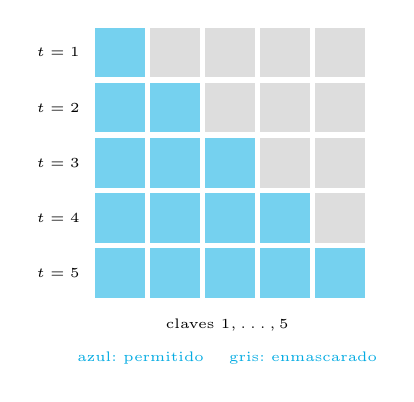
\begin{tikzpicture}[x=0.7cm,y=0.7cm]
					\foreach \r in {0,...,4}{
						\foreach \c in {0,...,4}{
							\ifnum\c>\r
								\fill[mitgray!40] (\c,-\r) rectangle ++(0.9,-0.9);
							\else
								\fill[UCMBlue!55] (\c,-\r) rectangle ++(0.9,-0.9);
							\fi
						}
						\node[font=\tiny, anchor=east] at (-0.1,-\r-0.45) {$t=\the\numexpr\r+1\relax$};
					}
					\node[font=\tiny] at (2.4,-5.4) {claves $1,\dots,5$};
					\node[font=\tiny, UCMBlue] at (2.4,-6.0) {azul: permitido \quad gris: enmascarado};
				\end{tikzpicture}
			\end{center}
		\end{column}
	\end{columns}
\end{frame}

\begin{frame}{Dropout sobre los Pesos y la Clase \texttt{CausalAttention}}
	\begin{columns}[T]
		\begin{column}{0.5\textwidth}
			\begin{block}{Dropout de atenci\'on}
				\small
				Despu\'es del softmax, durante el \textbf{entrenamiento}, cada peso se anula con probabilidad $p$ y los restantes se reescalan por $1/(1-p)$. En evaluaci\'on se desactiva.
			\end{block}
		\end{column}
		\begin{column}{0.47\textwidth}
			\begin{block}{\texttt{CausalAttention} en el lab}
				\small
				\begin{itemize}
					\item Proyecciones \texttt{nn.Linear} $\mathbf{W}_q,\mathbf{W}_k,\mathbf{W}_v$.
					\item Dimensi\'on de lote: \texttt{queries @ keys.transpose(1, 2)}.
					\item M\'ascara en \texttt{register\_buffer}: viaja a la GPU con el modelo pero no es un par\'ametro entrenable.
				\end{itemize}
			\end{block}
		\end{column}
	\end{columns}
	\begin{center}
		\small
		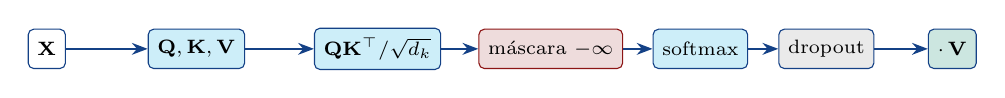
\begin{tikzpicture}[x=1cm,y=1cm]
			\node[smallbox] (x) at (0,0) {$\mathbf{X}$};
			\node[smallbox, fill=UCMBlue!20] (qkv) at (1.9,0) {$\mathbf{Q},\mathbf{K},\mathbf{V}$};
			\node[smallbox, fill=UCMBlue!20] (s) at (4.2,0) {$\mathbf{Q}\mathbf{K}^\top/\sqrt{d_k}$};
			\node[smallbox, fill=StanfordRed!15, draw=StanfordRed] (m) at (6.4,0) {m\'ascara $-\infty$};
			\node[smallbox, fill=UCMBlue!20] (sm) at (8.3,0) {softmax};
			\node[smallbox, fill=mitgray!25] (d) at (9.9,0) {dropout};
			\node[smallbox, fill=AccentGreen!20] (z) at (11.5,0) {$\cdot\,\mathbf{V}$};
			\foreach \a/\b in {x/qkv,qkv/s,s/m,m/sm,sm/d,d/z}{\draw[arr] (\a)--(\b);}
		\end{tikzpicture}
	\end{center}
\end{frame}

% =================================================================
\section{Atenci\'on Multi-Cabeza}

\begin{frame}{Atenci\'on Multi-Cabeza}
	Varias \emph{cabezas} atienden en paralelo a subespacios aprendidos distintos (relaciones sint\'acticas, de largo alcance, etc.).
	\formula{
		\[
		\mathbf{h}_i=f\big(\mathbf{W}^{(q)}_i\qv,\ \mathbf{W}^{(k)}_i\kv,\ \mathbf{W}^{(v)}_i\vv\big)\in\R^{p_v},\quad i=1,\dots,h
		\]
		\[
		\mathrm{MHA}(\qv,\kv,\vv)=\mathbf{W}_o\begin{bmatrix}\mathbf{h}_1\\ \vdots\\ \mathbf{h}_h\end{bmatrix}\in\R^{p_o},
		\qquad \mathbf{W}_o\in\R^{p_o\times h p_v}
		\]
	}
	\vspace{-0.2cm}
	\begin{columns}[T]
		\begin{column}{0.5\textwidth}
			\small
			\begin{itemize}
				\item $f$: atenci\'on de producto punto escalado.
				\item Para controlar el costo: $p_q=p_k=p_v=p_o/h$.
				\item As\'i el costo es similar al de una sola cabeza de dimensi\'on completa.
					\item En el lab: $p_o=$ \texttt{d\_out}, $p_v=$ \texttt{head\_dim} $=$ \texttt{d\_out}$/h$, $\mathbf{W}_o=$ \texttt{out\_proj}.
			\end{itemize}
		\end{column}
		\begin{column}{0.47\textwidth}
			\begin{center}
				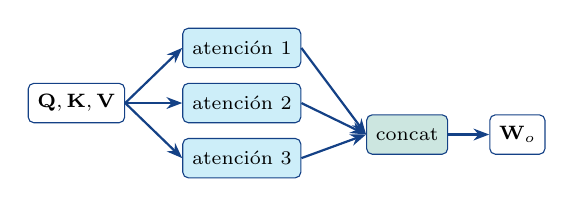
\begin{tikzpicture}[x=1cm,y=1cm]
					\node[smallbox] (in) at (0,0) {$\Q,\K,\Vm$};
					\foreach \i/\y in {1/1.1,2/0.4,3/-0.3}{
						\node[smallbox, fill=UCMBlue!20] (a\i) at (2.1,\y-0.4) {atenci\'on \i};
						\draw[arr] (in.east)--(a\i.west);
					}
					\node[smallbox, fill=AccentGreen!20] (cat) at (4.2,-0.4) {concat};
					\node[smallbox] (o) at (5.6,-0.4) {$\mathbf{W}_o$};
					\foreach \i in {1,2,3}{\draw[arr] (a\i.east)--(cat.west);}
					\draw[arr] (cat)--(o);
				\end{tikzpicture}
			\end{center}
		\end{column}
	\end{columns}
\end{frame}


\begin{frame}{Multi-Cabeza: de la Versi\'on Ingenua a la Eficiente}
	\begin{columns}[T]
		\begin{column}{0.48\textwidth}
			\begin{alertblock}{Ingenua: \texttt{MultiHeadAttentionWrapper}}
				\small
				$h$ instancias de \texttt{CausalAttention} en una \texttt{ModuleList}; se recorren con un \textbf{bucle} y se concatenan las salidas.
				La GPU queda subutilizada y la salida mide $h\cdot$\texttt{d\_out}.
			\end{alertblock}
		\end{column}
		\begin{column}{0.48\textwidth}
			\begin{block}{Eficiente: \texttt{MultiHeadAttention}}
				\small
				\textbf{Una} proyecci\'on grande de tama\~no \texttt{d\_out} y se \emph{divide} en $h$ cabezas con \texttt{view}: todas se calculan en un \'unico producto matricial por lote. \texttt{head\_dim = d\_out // num\_heads}.
			\end{block}
		\end{column}
	\end{columns}
	\vspace{0.1cm}
	\begin{center}
		\small
		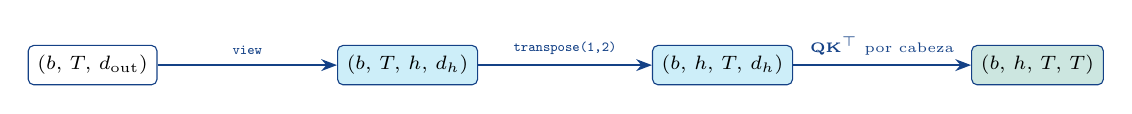
\begin{tikzpicture}[x=1cm,y=1cm]
			\node[smallbox] (a) at (0,0) {$(b,\,T,\,d_\text{out})$};
			\node[smallbox, fill=UCMBlue!20] (b) at (4,0) {$(b,\,T,\,h,\,d_h)$};
			\node[smallbox, fill=UCMBlue!20] (c) at (8,0) {$(b,\,h,\,T,\,d_h)$};
			\node[smallbox, fill=AccentGreen!20] (d) at (12,0) {$(b,\,h,\,T,\,T)$};
			\draw[arr] (a)--(b) node[midway,above,font=\tiny]{\texttt{view}};
			\draw[arr] (b)--(c) node[midway,above,font=\tiny]{\texttt{transpose(1,2)}};
			\draw[arr] (c)--(d) node[midway,above,font=\tiny]{$\mathbf{Q}\mathbf{K}^\top$ por cabeza};
		\end{tikzpicture}
	\end{center}
	\small
	Despu\'es: $(\text{pesos}\cdot\mathbf{V})\to(b,h,T,d_h)\xrightarrow{\texttt{transpose}}(b,T,h,d_h)\xrightarrow{\texttt{view}}(b,T,d_\text{out})\to\mathbf{W}_o$.
\end{frame}

\begin{frame}[fragile]{\texttt{MultiHeadAttention} en PyTorch (versi\'on del laboratorio)}
	\scriptsize
	\begin{tcolorbox}[colback=LightGray, colframe=UCMNavy, arc=3pt, boxsep=1pt]
\begin{verbatim}
class MultiHeadAttention(nn.Module):
    def __init__(self, d_in, d_out, context_length, dropout, num_heads, qkv_bias=False):
        super().__init__()
        assert d_out % num_heads == 0
        self.d_out, self.num_heads = d_out, num_heads
        self.head_dim = d_out // num_heads
        self.W_query = nn.Linear(d_in, d_out, bias=qkv_bias)   # idem W_key, W_value
        self.out_proj = nn.Linear(d_out, d_out)                # W_o
        self.dropout = nn.Dropout(dropout)
        self.register_buffer("mask", torch.triu(torch.ones(context_length, context_length), 1))

    def forward(self, x):
        b, T, _ = x.shape
        q = self.W_query(x).view(b, T, self.num_heads, self.head_dim).transpose(1, 2)
        k = ...  # igual con W_key;   v = ...  # igual con W_value   -> (b, heads, T, head_dim)

        scores = q @ k.transpose(2, 3)                         # (b, heads, T, T)
        scores.masked_fill_(self.mask.bool()[:T, :T], -torch.inf)
        w = self.dropout(torch.softmax(scores / k.shape[-1]**0.5, dim=-1))

        z = (w @ v).transpose(1, 2).contiguous().view(b, T, self.d_out)
        return self.out_proj(z)
\end{verbatim}
	\end{tcolorbox}
\end{frame}

% =================================================================
\section{Codificaci\'on Posicional}

\begin{frame}{La Auto-Atenci\'on No Conoce el Orden}
	Sin m\'ascara causal, permutar los tokens de entrada solo \textbf{permuta la salida}: sea $\boldsymbol{\Pi}$ una matriz de permutaci\'on,
	\formula{
		\small
		\[
		\softmax\!\Big(\tfrac{(\boldsymbol\Pi\mathbf{Q})(\boldsymbol\Pi\mathbf{K})^\top}{\sqrt d}\Big)\boldsymbol\Pi\mathbf{V}
		=\boldsymbol\Pi\,\softmax\!\Big(\tfrac{\mathbf{Q}\mathbf{K}^\top}{\sqrt d}\Big)\boldsymbol\Pi^\top\boldsymbol\Pi\mathbf{V}
		=\boldsymbol\Pi\,\mathrm{SA}(\mathbf{X})
		\]
	}
	\vspace{-0.2cm}
	\begin{columns}[T]
		\begin{column}{0.5\textwidth}
			\begin{alertblock}{Consecuencia}
				\small
				``el perro mordi\'o al hombre'' y ``el hombre mordi\'o al perro'' producen los mismos vectores (reordenados): el modelo \textbf{no distingue} el orden.
			\end{alertblock}
		\end{column}
		\begin{column}{0.47\textwidth}
			\begin{block}{Soluci\'on}
				\small
				Sumar la codificaci\'on posicional: con ella, $\mathrm{SA}(\boldsymbol\Pi\mathbf{X}+\mathbf{P})\neq\boldsymbol\Pi\,\mathrm{SA}(\mathbf{X}+\mathbf{P})$, porque al reordenar cada token recibe la posici\'on de su \emph{nuevo} lugar.
				\smallskip

				(Ejercicio 3 del laboratorio.)
			\end{block}
		\end{column}
	\end{columns}
\end{frame}

\begin{frame}{Codificaci\'on Posicional}
	La auto-atenci\'on es invariante al orden $\Rightarrow$ se \emph{suma} una matriz $\mathbf{P}\in\R^{n\times d}$ a la entrada: $\mathbf{X}+\mathbf{P}$.
	\formula{
		\[
		p_{i,2j}=\sin\!\left(\frac{i}{10000^{2j/d}}\right),\qquad
		p_{i,2j+1}=\cos\!\left(\frac{i}{10000^{2j/d}}\right)
		\]
	}
	\vspace{-0.3cm}
	\begin{columns}[T]
		\begin{column}{0.5\textwidth}
			\begin{center}
				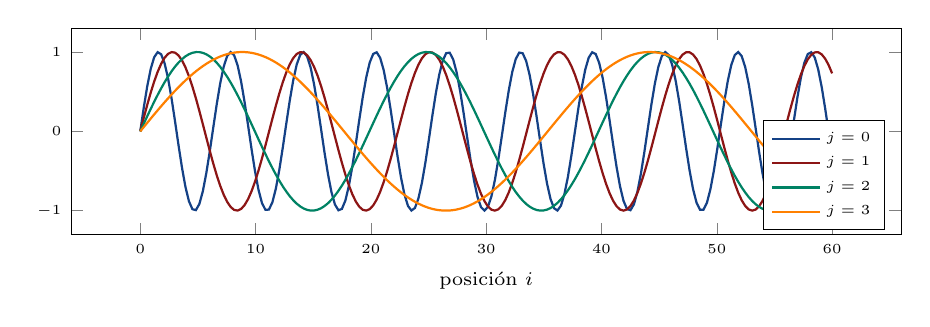
\begin{tikzpicture}
					\begin{axis}[width=\textwidth, height=4.2cm, xlabel={posici\'on $i$}, domain=0:60, samples=200,
						legend style={font=\tiny, at={(0.98,0.02)}, anchor=south east},
						tick label style={font=\tiny}, label style={font=\scriptsize}, ymin=-1.3, ymax=1.3]
						\addplot[thick, UCMNavy] {sin(deg(x))};
						\addplot[thick, StanfordRed] {sin(deg(x*0.5623))};
						\addplot[thick, AccentGreen] {sin(deg(x*0.3162))};
						\addplot[thick, orange] {sin(deg(x*0.1778))};
						\legend{$j=0$,$j=1$,$j=2$,$j=3$}
					\end{axis}
				\end{tikzpicture}
			\end{center}
			{\tiny Ejemplo con $d=32$: columnas de $\sin$ de frecuencia decreciente.}
		\end{column}
		\begin{column}{0.47\textwidth}
			\begin{block}{Propiedad de posici\'on relativa}
				\small
				Con $\omega_j=10000^{-2j/d}$, un giro fijo depende solo del desfase $\delta$:
				\[
				\begin{bmatrix}\cos\delta\omega_j & \sin\delta\omega_j\\ -\sin\delta\omega_j & \cos\delta\omega_j\end{bmatrix}
				\begin{bmatrix}p_{i,2j}\\ p_{i,2j+1}\end{bmatrix}=
				\begin{bmatrix}p_{i+\delta,2j}\\ p_{i+\delta,2j+1}\end{bmatrix}
				\]
				El modelo puede aprender a atender por \textbf{offset relativo}.
			\end{block}
		\end{column}
	\end{columns}
\end{frame}


% =================================================================
\section{El Transformer}

\begin{frame}{La Arquitectura Transformer}
	Vaswani et al.\ (2017), \emph{Attention is all you need}: codificador--decodificador \textbf{solo con atenci\'on y capas feed-forward}, sin convoluci\'on ni recurrencia.
	\begin{center}
		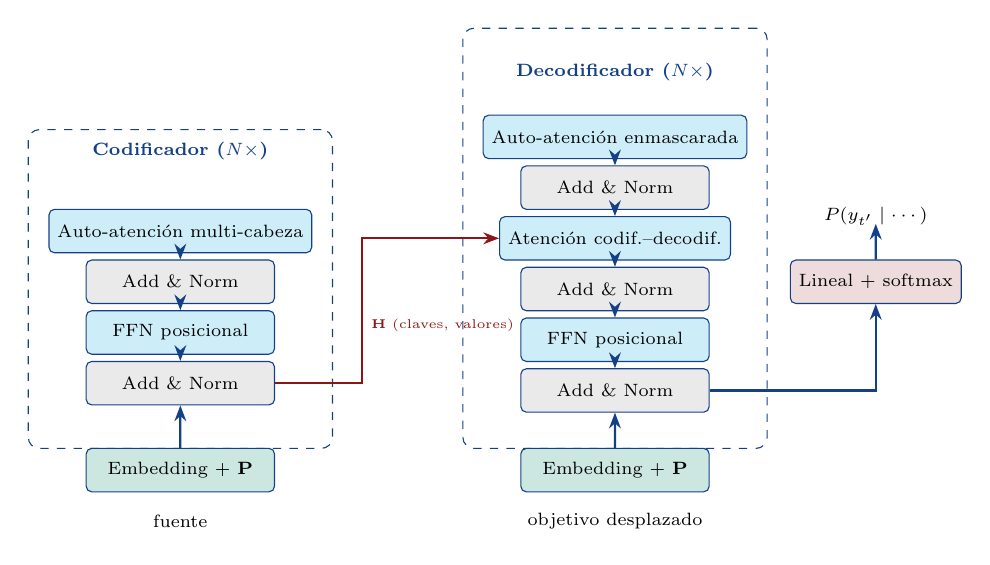
\begin{tikzpicture}[x=1cm,y=1cm, scale=0.92, transform shape]
			% Encoder
			\node[draw=UCMNavy, dashed, rounded corners, minimum width=4.2cm, minimum height=4.4cm] at (0,1.1) {};
			\node[font=\scriptsize\bfseries, UCMNavy] at (0,3.0) {Codificador ($N\times$)};
			\node[box, fill=UCMBlue!20] (ea) at (0,1.9) {Auto-atenci\'on multi-cabeza};
			\node[box, fill=mitgray!25] (en1) at (0,1.2) {Add \& Norm};
			\node[box, fill=UCMBlue!20] (ef) at (0,0.5) {FFN posicional};
			\node[box, fill=mitgray!25] (en2) at (0,-0.2) {Add \& Norm};
			\draw[arr] (ea)--(en1); \draw[arr] (en1)--(ef); \draw[arr] (ef)--(en2);
			\node[box, fill=AccentGreen!20] (ee) at (0,-1.4) {Embedding + $\mathbf{P}$};
			\draw[arr] (ee)--(en2);
			\node[font=\scriptsize] at (0,-2.1) {fuente};
			% Decoder
			\node[draw=UCMNavy, dashed, rounded corners, minimum width=4.2cm, minimum height=5.8cm] at (6,1.8) {};
			\node[font=\scriptsize\bfseries, UCMNavy] at (6,4.1) {Decodificador ($N\times$)};
			\node[box, fill=UCMBlue!20] (da) at (6,3.2) {Auto-atenci\'on enmascarada};
			\node[box, fill=mitgray!25] (dn1) at (6,2.5) {Add \& Norm};
			\node[box, fill=UCMBlue!20] (dc) at (6,1.8) {Atenci\'on codif.--decodif.};
			\node[box, fill=mitgray!25] (dn2) at (6,1.1) {Add \& Norm};
			\node[box, fill=UCMBlue!20] (df) at (6,0.4) {FFN posicional};
			\node[box, fill=mitgray!25] (dn3) at (6,-0.3) {Add \& Norm};
			\draw[arr] (da)--(dn1); \draw[arr] (dn1)--(dc); \draw[arr] (dc)--(dn2);
			\draw[arr] (dn2)--(df); \draw[arr] (df)--(dn3);
			\node[box, fill=AccentGreen!20] (de) at (6,-1.4) {Embedding + $\mathbf{P}$};
			\draw[arr] (de)--(dn3);
			\node[font=\scriptsize] at (6,-2.1) {objetivo desplazado};
			% enc -> dec cross
			\draw[arr, StanfordRed] (en2.east) -- ++(1.2,0) |- (dc.west) node[pos=0.2, right, font=\tiny, StanfordRed]{$\mathbf{H}$ (claves, valores)};
			% output
			\node[box, fill=StanfordRed!15, minimum width=2cm] (out) at (9.6,1.2) {Lineal + softmax};
			\draw[arr] (dn3.east) -| (out.south);
			\node[font=\scriptsize] at (9.6,2.1) {$P(y_{t'}\mid\cdots)$};
			\draw[arr] (out)--(9.6,2.0);
		\end{tikzpicture}
	\end{center}
\end{frame}

\begin{frame}{Bloques del Codificador y del Decodificador}
	\begin{columns}[T]
		\begin{column}{0.5\textwidth}
			\begin{block}{Bloque del codificador}
				\small
				\[
				\mathbf{Z}=\mathrm{LN}\big(\mathbf{X}+\mathrm{Drop}(\mathrm{MHA}(\mathbf{X},\mathbf{X},\mathbf{X}))\big)
				\]
				\[
				\mathbf{Y}=\mathrm{LN}\big(\mathbf{Z}+\mathrm{Drop}(\mathrm{FFN}(\mathbf{Z}))\big)
				\]
			\end{block}
			\small
			Cada subcapa entrega dimensi\'on $d$ para poder sumar el residual. El bloque \textbf{no cambia la forma} del tensor.
		\end{column}
		\begin{column}{0.5\textwidth}
			\begin{block}{Bloque del decodificador}
				\scriptsize
				\[
				\mathbf{Z}_1=\mathrm{LN}\big(\mathbf{X}+\mathrm{Drop}(\mathrm{MHA}_{\text{enmasc.}}(\mathbf{X},\mathbf{X},\mathbf{X}))\big)
				\]
				\[
				\mathbf{Z}_2=\mathrm{LN}\big(\mathbf{Z}_1+\mathrm{Drop}(\mathrm{MHA}(\mathbf{Z}_1,\mathbf{H},\mathbf{H}))\big)
				\]
				\[
				\mathbf{Z}_3=\mathrm{LN}\big(\mathbf{Z}_2+\mathrm{Drop}(\mathrm{FFN}(\mathbf{Z}_2))\big)
				\]
			\end{block}
			\small
			$\mathbf{H}$ = salida del codificador, usada como claves y valores.
		\end{column}
	\end{columns}
	\vspace{0.2cm}
	\begin{alertblock}{Embeddings}
		\small
		Se multiplican por $\sqrt d$ antes de sumar $\mathbf{P}$ (cuyos valores est\'an en $[-1,1]$), para que la posici\'on no domine la se\~nal del token.
	\end{alertblock}
\end{frame}

\begin{frame}{FFN Posicional, Residuales y Normalizaci\'on de Capa}
	\begin{columns}[T]
		\begin{column}{0.48\textwidth}
			\begin{block}{FFN posicional}
				\small
				El \textbf{mismo} MLP de dos capas se aplica a cada posici\'on por separado:
				\[
				\mathrm{FFN}(\mathbf{x})=\max(0,\mathbf{x}\mathbf{W}_1+\mathbf{b}_1)\mathbf{W}_2+\mathbf{b}_2
				\]
				Entradas id\'enticas en posiciones distintas dan salidas id\'enticas; la mezcla entre posiciones la hace solo la atenci\'on.
			\end{block}
		\end{column}
		\begin{column}{0.48\textwidth}
			\begin{block}{Add \& Norm}
				\small
				\begin{itemize}
					\item \textbf{Residual}: $\mathbf{x}+\text{subcapa}(\mathbf{x})$ facilita el flujo de gradientes en pilas profundas.
					\item \textbf{Layer norm}: normaliza sobre las \emph{caracter\'isticas} de cada ejemplo.
					\item Batch norm normaliza sobre el lote; en secuencias de largo variable es inestable, por eso se prefiere layer norm.
				\end{itemize}
			\end{block}
		\end{column}
	\end{columns}
\end{frame}

\begin{frame}{Los Tres Tipos de Atenci\'on en el Transformer}
	\begin{center}
		\small
		\begin{tabular}{p{3.8cm}p{2.4cm}p{2.4cm}p{3.2cm}}
			\toprule
			Capa & Consultas & Claves / valores & M\'ascara\\
			\midrule
			Auto-atenci\'on del codificador & codificador & codificador & padding\\
			Auto-atenci\'on del decodificador & decodificador & decodificador & causal + padding\\
			Atenci\'on codificador--decodificador & decodificador & salida del codificador $\mathbf{H}$ & padding de la fuente\\
			\bottomrule
		\end{tabular}
	\end{center}
	\begin{block}{Configuraci\'on del ejemplo EN$\to$FR de d2l}
		\small
		2 bloques de codificador y 2 de decodificador, 4 cabezas, dimensi\'on 256, dropout 0.2, lr $=0.001$, 30 \'epocas, recorte de gradiente 1.
		Los mapas de atenci\'on del codificador--decodificador muestran el alineamiento objetivo $\to$ fuente.
	\end{block}
	\begin{alertblock}{En la pr\'actica}
		\small
		Muchos modelos usan solo el codificador (BERT) o solo el decodificador (GPT): ver la secci\'on de preentrenamiento.
	\end{alertblock}
\end{frame}

% =================================================================
\section{Transformers para Visi\'on}

\begin{frame}{Vision Transformer (ViT)}
	Una imagen se trata como una \textbf{secuencia de parches}, igual que el texto es una secuencia de tokens.
	\begin{columns}[T]
		\begin{column}{0.5\textwidth}
			\begin{enumerate}
				\small
				\item Imagen $h\times w\times c$ dividida en parches $p\times p$: $m=hw/p^2$.
				\item Cada parche aplanado ($cp^2$) se proyecta linealmente a $\R^d$ (equivale a una convoluci\'on con \emph{kernel} y \emph{stride} $=p$).
				\item Se antepone un token \texttt{<cls>} y se suman embeddings posicionales aprendibles.
				\item Pila de bloques Transformer (codificador).
				\item Cabeza de clasificaci\'on sobre la salida de \texttt{<cls>}.
			\end{enumerate}
			\formula{
				\small
				$\mathbf{Z}_0=[\mathbf{x}_{\text{cls}};\mathbf{X}_p\mathbf{E}]+\mathbf{E}_{\text{pos}}$
			}
		\end{column}
		\begin{column}{0.47\textwidth}
			\begin{center}
				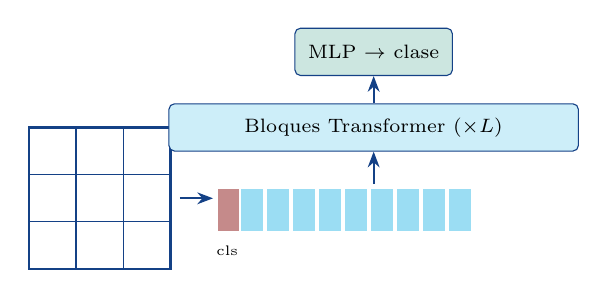
\begin{tikzpicture}[x=0.6cm,y=0.6cm]
					\draw[thick, UCMNavy] (0,0) rectangle (3,3);
					\foreach \i in {1,2}{\draw[UCMNavy] (\i,0)--(\i,3); \draw[UCMNavy] (0,\i)--(3,\i);}
					\foreach \i in {0,...,8}{
						\pgfmathsetmacro{\x}{4.5+\i*0.55}
						\fill[UCMBlue!40] (\x,0.8) rectangle ++(0.45,0.9);
					}
					\fill[StanfordRed!50] (4,0.8) rectangle ++(0.45,0.9);
					\node[font=\tiny] at (4.2,0.4) {cls};
					\draw[arr] (3.2,1.5)--(3.9,1.5);
					\node[box, minimum width=5.2cm, fill=UCMBlue!20] (t) at (7.3,3.0) {Bloques Transformer ($\times L$)};
					\draw[arr] (7.3,1.8)--(t.south);
					\node[box, minimum width=2cm, fill=AccentGreen!20] (c) at (7.3,4.6) {MLP $\to$ clase};
					\draw[arr] (t.north)--(c.south);
				\end{tikzpicture}
			\end{center}
		\end{column}
	\end{columns}
\end{frame}

\begin{frame}{ViT: Detalles y Lecciones}
	\begin{columns}[T]
		\begin{column}{0.5\textwidth}
			\begin{block}{Bloque \emph{pre-norm}}
				\small
				\[
				\mathbf{Z}'=\mathbf{Z}+\mathrm{MSA}(\mathrm{LN}(\mathbf{Z}))
				\]
				\[
				\mathbf{Z}''=\mathbf{Z}'+\mathrm{MLP}(\mathrm{LN}(\mathbf{Z}'))
				\]
				La normalizaci\'on va \emph{antes} de cada subcapa (entrena mejor que post-norm). El MLP usa GELU.
			\end{block}
			\begin{block}{Ejemplo d2l (Fashion-MNIST)}
				\small
				Imagen 96, parche 16 $\Rightarrow m=36$ parches; 8 cabezas, 2 bloques, 512 ocultas.
			\end{block}
		\end{column}
		\begin{column}{0.47\textwidth}
			\begin{alertblock}{Sesgo inductivo}
				\small
				En conjuntos peque\~nos o medianos, ViT \textbf{no supera} a una ResNet: le faltan la localidad y la invarianza a traslaciones de la convoluci\'on.
			\end{alertblock}
			\begin{block}{Con datos masivos}
				\small
				Con modelos y conjuntos mucho m\'as grandes (cientos de millones de im\'agenes), ViT supera claramente a las ResNet.
			\end{block}
			\small
			Costo cuadr\'atico en el n\'umero de parches. Variantes: DeiT (eficiencia de datos), Swin (ventanas desplazadas).
		\end{column}
	\end{columns}
\end{frame}

% =================================================================
\section{Preentrenamiento a Gran Escala}

\begin{frame}{Tres Familias de Transformers Preentrenados}
	\begin{center}
		\small
		\begin{tabular}{p{2.6cm}p{2.7cm}p{3.1cm}p{4.2cm}}
			\toprule
			& \textbf{Solo codificador} & \textbf{Codificador--decodificador} & \textbf{Solo decodificador}\\
			\midrule
			Ejemplo & BERT & T5 & GPT, GPT-2, GPT-3\\
			Atenci\'on & bidireccional & bidireccional + causal & causal\\
			Preentrenamiento & lenguaje enmascarado (MLM) & corrupci\'on de tramos & modelado de lenguaje autorregresivo\\
			Uso t\'ipico & clasificaci\'on, etiquetado & texto a texto (traducci\'on, resumen) & generaci\'on, \emph{in-context learning}\\
			\bottomrule
		\end{tabular}
	\end{center}
	\begin{block}{Idea com\'un}
		\small
		Preentrenar con texto sin etiquetas (autosupervisi\'on) y luego \textbf{adaptar} a tareas espec\'ificas: ajuste fino o, en modelos muy grandes, solo \emph{prompting}.
	\end{block}
\end{frame}

\begin{frame}{BERT, T5 y GPT: Objetivos de Preentrenamiento}
	\begin{columns}[T]
		\begin{column}{0.33\textwidth}
			\begin{block}{BERT (MLM)}
				\scriptsize
				Se reemplazan tokens al azar por \texttt{<mask>} y se predicen con entrop\'ia cruzada, usando contexto a ambos lados.

				\medskip
				``I \texttt{<mask>} this red car'' $\to$ \emph{love}

				\medskip
				Ajuste fino: capa nueva sobre \texttt{<cls>}, entrenada junto con los par\'ametros preentrenados.
			\end{block}
		\end{column}
		\begin{column}{0.33\textwidth}
			\begin{block}{T5 (texto a texto)}
				\scriptsize
				Tramos consecutivos enmascarados comparten un token centinela; el decodificador los reconstruye.

				\medskip
				Entrada: ``I \texttt{<X>} this \texttt{<Y>}''\\
				Salida: ``\texttt{<X>} love \texttt{<Y>} red car \texttt{<Z>}''

				\medskip
				Toda tarea es texto $\to$ texto, sin capas espec\'ificas.
			\end{block}
		\end{column}
		\begin{column}{0.33\textwidth}
			\begin{block}{GPT (autorregresivo)}
				\scriptsize
				El objetivo es la entrada desplazada un token; atenci\'on causal.
				\[
				\max_\theta \sum_t \log p_\theta(x_t\mid x_{<t})
				\]
				GPT-2: 1.5\,B par\'ametros; ejecuta tareas sin actualizar pesos. GPT-3: \emph{zero-, one-} y \emph{few-shot} v\'ia contexto.
			\end{block}
		\end{column}
	\end{columns}
\end{frame}

\begin{frame}{Escalamiento}
	\begin{itemize}
		\item Kaplan et al.\ (2020): el desempe\~no sigue una \textbf{ley de potencias} en el tama\~no del modelo, el tama\~no del conjunto de datos y el c\'omputo.
		\item Los modelos m\'as grandes son m\'as \textbf{eficientes en muestras}.
		\item Capacidades nuevas aparecen con la escala: \emph{in-context learning} sin actualizar par\'ametros.
	\end{itemize}
	\begin{center}
		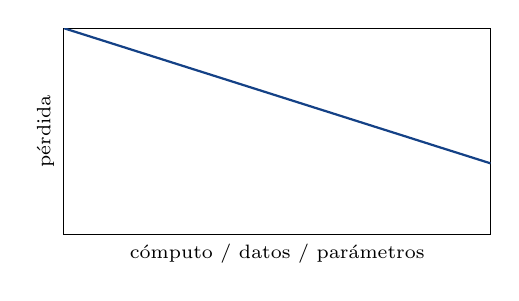
\begin{tikzpicture}
			\begin{axis}[width=7cm, height=4.2cm, xmode=log, ymode=log, xlabel={c\'omputo / datos / par\'ametros},
				ylabel={p\'erdida}, xmin=1, xmax=1000, ymin=0.5, ymax=20, tick label style={font=\tiny},
				label style={font=\scriptsize}, ticks=none]
				\addplot[thick, UCMNavy, domain=1:1000] {20*x^(-0.35)};
			\end{axis}
		\end{tikzpicture}

		{\tiny Esquema cualitativo de una ley de potencias (recta en escala log--log); no son datos reales.}
	\end{center}
\end{frame}

% =================================================================
\section{Laboratorio 3.3}

\begin{frame}{Laboratorio 3.3: de las Diapositivas al C\'odigo}
	\small
	Cuaderno \texttt{labs/3.3\_AtencionPyTorch.ipynb} (basado en el cap.\ 3 de \emph{Build a Large Language Model From Scratch}, S.\ Raschka).
	\begin{center}
		\scriptsize
		\begin{tabular}{p{4.2cm}p{4.3cm}p{4.2cm}}
			\toprule
			\textbf{Secci\'on del lab} & \textbf{Qu\'e se implementa} & \textbf{Diapositivas}\\
			\midrule
			1. Auto-atenci\'on simple & $\mathbf{Z}=\softmax(\mathbf{X}\mathbf{X}^\top)\mathbf{X}$ con bucles y en forma matricial & Auto-atenci\'on simple\\
			2. Pesos entrenables & $\mathbf{W}_q,\mathbf{W}_k,\mathbf{W}_v$; \texttt{SelfAttention\_v1/v2}; experimento de $\sqrt{d_k}$ & Producto punto escalado; auto-atenci\'on con pesos\\
			3. Atenci\'on causal & m\'ascara $-\infty$, dropout, \texttt{CausalAttention} & M\'ascara antes del softmax; m\'ascara triangular; dropout\\
			4. Multi-cabeza & \texttt{ModuleList} vs.\ divisi\'on de pesos con \texttt{view} & Ingenua vs.\ eficiente; c\'odigo\\
			\bottomrule
		\end{tabular}
	\end{center}
\end{frame}

\begin{frame}{Actividad del Laboratorio y D\'onde Repasarla}
	\begin{enumerate}
		\item \textbf{Atenci\'on escalada a mano}: implementar $\softmax(\mathbf{Q}\mathbf{K}^\top/\sqrt{d_k})\mathbf{V}$ con m\'ascara opcional y compararla con \texttt{F.scaled\_dot\_product\_attention}. \emph{(Producto punto escalado, m\'ascara causal.)}
		\item \textbf{Comparar con \texttt{nn.MultiheadAttention}}: copiar sus pesos a nuestra clase y verificar que coinciden. \emph{(Multi-cabeza: $\mathbf{W}_o$ y \texttt{head\_dim}.)}
		\item \textbf{Equivarianza a permutaciones} y \textbf{codificaci\'on posicional sinusoidal}: mostrar que sin posici\'on el orden no importa y que con ella s\'i. \emph{(La auto-atenci\'on no conoce el orden; codificaci\'on posicional.)}
		\item \textbf{Mini bloque Transformer}: MHA + FFN con residuales y LayerNorm. \emph{(Bloques del codificador y del decodificador; FFN, Add \& Norm.)}
	\end{enumerate}
	\begin{alertblock}{Convenci\'on de m\'ascaras}
		\small
		En el lab la m\'ascara booleana vale \texttt{True} donde \textbf{no} se debe atender, y se aplica con \texttt{masked\_fill(..., -torch.inf)}. En la diapositiva de \emph{masked softmax} (d2l) se usan longitudes v\'alidas y un valor $-10^{6}$; es la misma idea.
	\end{alertblock}
\end{frame}

% =================================================================
\section{Conclusiones}

\begin{frame}{Resumen}
	\begin{columns}[T]
		\begin{column}{0.5\textwidth}
			\begin{block}{Atenci\'on}
				\small
				\begin{itemize}
					\item Promedio ponderado de \textbf{valores}, con pesos que salen de la similitud \textbf{consulta--clave} (softmax).
					\item Producto punto escalado: $\softmax(\Q\K^\top/\sqrt d)\Vm$.
					\item Atenci\'on aditiva para dimensiones distintas.
					\item Auto-atenci\'on: $\mathbf{Q},\mathbf{K},\mathbf{V}$ salen de la misma secuencia; m\'ascara causal para modelos autorregresivos.
					\item Multi-cabeza: varios subespacios en paralelo.
				\end{itemize}
			\end{block}
		\end{column}
		\begin{column}{0.47\textwidth}
			\begin{block}{Transformer}
				\small
				\begin{itemize}
					\item Auto-atenci\'on: paralelismo y camino $\mathcal{O}(1)$, a costo $\mathcal{O}(n^2d)$.
					\item Codificaci\'on posicional para recuperar el orden.
					\item Residuales + layer norm + FFN posicional.
					\item Decodificador con m\'ascara causal.
					\item Base de BERT, T5, GPT y ViT.
				\end{itemize}
			\end{block}
		\end{column}
	\end{columns}
\end{frame}

\begin{frame}{Ejercicios Te\'oricos Sugeridos}
	\begin{enumerate}
		\item Demuestre que con $a(\qv,\kv_i)=\qv^\top\kv_i$ y $\kv_i=\vv_i$ se cumple $\nabla_{\qv}\mathrm{Attention}(\qv,\mathcal{D})=\mathrm{Cov}_{p(\kv_i;\qv)}[\kv_i]$.
		\item Muestre que $\mathrm{Var}(\qv^\top\kv)=d$ si las componentes son independientes con media 0 y varianza 1.
		\item Reemplace la atenci\'on aditiva por producto punto escalado en el modelo de Bahdanau. ¿Cambia la eficiencia del entrenamiento?
		\item Visualice los pesos por cabeza en un Transformer entrenado. ¿Qu\'e cabezas podr\'ian podarse?
		\item Proponga una codificaci\'on posicional aprendible y comp\'arela con la sinusoidal.
		\item En ViT, sustituya el token \texttt{<cls>} por \emph{mean pooling}. ¿Qu\'e cambia?
	\end{enumerate}
	\vfill
	{\scriptsize Referencia: Zhang et al., \emph{Dive into Deep Learning}, cap.\ 11, \texttt{d2l.ai}. Vaswani et al.\ (2017); Bahdanau et al.\ (2014); Dosovitskiy et al.\ (2020); Devlin et al.\ (2018).}
\end{frame}

\end{document}
